\section{Derivation of Fundamental Constants}
%=============================================================================

%-----------------------------------------------------------------------------
\subsection{\texorpdfstring{The Geometric Scale $\phiz$}{The Geometric Scale phi0}}
%-----------------------------------------------------------------------------

\begin{theorem}{Existence and Uniqueness of $\phiz$}{phi0}
From Axioms A3 and A4, the geometric scale is uniquely determined:
\begin{equation}
    \phiz = \phitree + \deltatop = \frac{1}{6\pi} + \frac{3}{256\pi^4} = \num[round-mode=places,round-precision=17]{\TFPTvarphiZeroNum}
\end{equation}
\end{theorem}

\begin{proof}
From A3 ($\eta$-gluing): the M\"obius double cover contributes two physical boundary
cycles ($2\pi+2\pi$) plus a discrete seam gluing term ($2\pi$), giving
$R_{\text{total}}=6\pi$. The closure normalization $\chi = \varphi R = 1$
yields $\phitree = 1/(6\pi)$.
Here $\varphi$ is the dimensionless geometry modulus of the M\"obius reduction; the
normalization fixes its scale and can be taken as an explicit geometric-closure axiom.
Physical predictions depend only on dimensionless ratios and the discrete increments.

From A4: the unique gauge-invariant correction at leading order is 
$\deltatop = 48\cthree^4 = 3/(256\pi^4)$.
\end{proof}

\begin{tcolorbox}[colback=gray!5, colframe=gray!60, breakable,
    title={\textbf{Dictionary: $\beta_{\text{rad}}$ and Canonical Consequences}}, fonttitle=\bfseries\small]
\textbf{Definition (notation):}
\[
\beta_{\text{rad}} := \frac{\phiz}{4\pi}.
\]
\textit{Note:} dimensionless; equals the birefringence angle in radians for the minimal topological excursion $\Delta a_{\text{top}}=\phiz$.

\textbf{Immediate algebraic consequences:}
\begin{equation}
    \phiz = 4\pi\beta_{\text{rad}}, 
    \qquad 
    \beta_{\text{deg}} := \frac{180}{\pi}\,\beta_{\text{rad}}.
\end{equation}
\begin{equation}
    \gagg = -4\cthree = -\frac{1}{2\pi},
    \qquad
    \deltatop = 48\cthree^4 = \frac{3}{256\pi^4}.
\end{equation}

\textbf{Remark:} Many later ``$\beta_{\text{rad}}$-centric'' relations are compact rewrites of earlier definitions. 
We catalogue their logical status (definition vs.\ consequence vs.\ lemma vs.\ prediction) in Appendix~\ref{app:identities}.
\end{tcolorbox}

% Suite-extracted invariant table (high precision)
\TFPTCoreInvariantTable

%-----------------------------------------------------------------------------
\subsection{The Cubic Fixed-Point Equation (CFE)}
%-----------------------------------------------------------------------------

\begin{definition}{Effective Potential Parameters}{params}
From the 11D Chern--Simons reduction (A5) and modulus-closure structure (A6):
\begin{align}
    A &= 2\cthree^3 = \frac{1}{256\pi^3} \approx 1.2598 \times 10^{-4}\\[0.5em]
    \mathcal{K} &= \frac{\bone}{2\pi}\ln\frac{1}{\phiz} \approx 1.9147
\end{align}
\textbf{Notation:} We use $\mathcal{K}$ (calligraphic) for this CFE parameter to 
distinguish it from $\kappa^2 = 8\pi G$ (gravitational coupling) and the contorsion tensor $K$.
\end{definition}

\begin{tcolorbox}[colback=gray!5, colframe=gray!60,
    title={\textbf{Lemma (Geometric Fixing of the Log)}}, fonttitle=\bfseries\small]
In TFPT the one-loop logarithm is the ratio of a UV scale to a geometrically fixed IR scale:
\begin{equation}
    \ln\frac{1}{\phiz} = \ln\frac{\Lambda}{\mu_{\text{geo}}}.
\end{equation}
Here $\mu_{\text{geo}} \equiv \ell_{\text{geo}}^{-1}$ is fixed by the M\"obius curvature
normalization ($R_{\text{total}}=6\pi$), and $\phiz = \ell_{\text{UV}}/\ell_{\text{geo}}$.
Thus the renormalization point is not a free choice but is geometrically determined.
\end{tcolorbox}

\begin{tcolorbox}[colback=yellow!3, colframe=yellow!60!black,
    title={\textbf{Quantization and scheme declaration}}, fonttitle=\bfseries\small]
\textbf{Scheme:} dimensional regularization, background-field gauge, $\overline{\mathrm{MS}}$.
\textbf{Coefficient policy:} we postulate the fixed coefficients in
$U(\alpha)=\frac{A}{4}\alpha^4-\frac{2}{3}A\cthree^3\alpha^3-8A\bone\cthree^6 L\,\alpha+\ldots$
within the declared scheme.
\textbf{Status:} postulated input, audited for internal consistency across suite implementations;
a full background-field derivation is deferred.
\end{tcolorbox}

\begin{tcolorbox}[colback=yellow!5, colframe=yellow!60!black,
    title={\textbf{Status of the $\alpha^2$ term: Renormalization Condition Contract}}, fonttitle=\bfseries\small]

The $\alpha^2$ term in the CFE is \emph{scheme dependent}: it appears generically in
any one-loop background-field determinant but is removable by a declared renormalization
condition.  TFPT fixes this degree of freedom as follows.

\textbf{1.\ Generic occurrence:}
A quadratic term $\alpha^2$ appears generically in the one-loop determinant
of any toy background-field calculation.

\textbf{2.\ Declared contract:}
We fix a counterterm $\delta c_2 = -c_2$ at the geometric reference point
$\mu_{\mathrm{geo}}$, so the stationarity polynomial has no residual $\alpha^2$
in the declared scheme.
This is a renormalization condition (not a Ward-identity theorem).

\textbf{3.\ Invariance test:}
Under scheme shifts $\delta L \in [-0.5,+0.5]$, the compensating counterterm
$C_{\mathrm{ct}}$ absorbs the shift exactly; the compensated $\alpha^\star$ is
invariant to $< 10^{-70}$~ppm (algebraic identity in the policy).

\textbf{4.\ Robustness and scheme-shift compensated invariance:}
A separate robustness scan perturbs $\epsilon_2\in[10^{-12},10^{-8}]$; the resulting
$|\Delta\alpha^{-1}|$ stays below 1~ppm for $\epsilon_2<1.58\times 10^{-10}$, i.e.\
several orders of magnitude above any physical back-coupling.
The scheme-shift compensated invariance audit confirms that the full counterterm
chain is algebraically exact, not a numerical coincidence.

\textbf{Evidence:} \texttt{alpha2\_contract\_and\_scheme\_invariance\_audit},
\texttt{alpha2\_renorm\_condition\_audit}, \texttt{alpha2\_term\_robustness\_scan},
\texttt{alpha2\_coefficient\_policy\_referee\_exit\_gate\_v28} (all PASS).
\end{tcolorbox}

\begin{figure}[H]
\centering
\begin{tikzpicture}
\begin{groupplot}[
    group style={group size=2 by 1, horizontal sep=1.8cm},
    width=0.44\linewidth, height=0.36\linewidth
]
\nextgroupplot[
    xlabel={$\delta L$},
    ylabel={$C_{\mathrm{ct}}$},
    title={Compensating counterterm},
    grid=major,
    scaled y ticks=base 10:-8,
]
\addplot+[mark=o, thick] coordinates {
    (-0.5,-6.51e-08) (-0.2,-2.60e-08) (-0.1,-1.30e-08)
    (-0.05,-6.51e-09) (0.0,0.0) (0.05,6.51e-09)
    (0.1,1.30e-08) (0.2,2.60e-08) (0.5,6.51e-08)
};

\nextgroupplot[
    xlabel={$\delta L$},
    ylabel={residual (ppm)},
    title={Residual after compensation},
    grid=major,
    ymode=log,
    ymin=1e-78, ymax=1e-74,
]
\addplot+[mark=square, thick] coordinates {
    (-0.5,1.65e-76) (-0.2,3.74e-77) (-0.1,1.99e-76)
    (-0.05,9.84e-77) (0.05,9.84e-77) (0.1,2.37e-76)
    (0.2,3.74e-77) (0.5,2.72e-76)
};
\end{groupplot}
\end{tikzpicture}
\caption{Scheme-shift invariance of the $\alpha^2$ renorm contract.
  Left: counterterm scales linearly with $\delta L$.
  Right: compensated residual is numerically zero ($< 10^{-76}$~ppm).}
\label{fig:alpha2-contract}
\end{figure}

\begin{figure}[H]
\centering
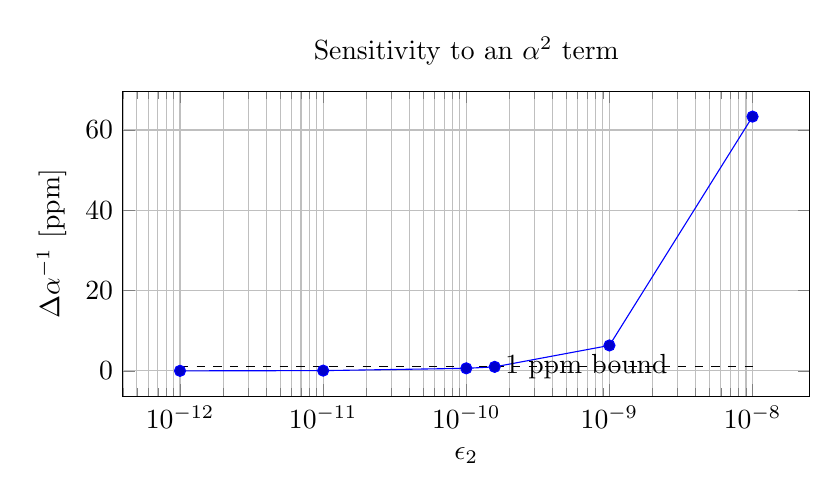
\begin{tikzpicture}
\begin{axis}[
  width=0.85\linewidth,
  height=0.45\linewidth,
  grid=both,
  xlabel={$\epsilon_2$},
  ylabel={$\Delta \alpha^{-1}$ [ppm]},
  xmode=log,
  title={Sensitivity to an $\alpha^2$ term},
]
\addplot table[row sep=\\] {
eps ppm\\
1e-12 0.006332528061424504\\
1e-11 0.06332528424435171\\
1e-10 0.6332532054543387\\
1.579153968e-10 1.0\\
1e-9 6.332568355779471\\
1e-8 63.32931383533495\\
};
\addplot[black, dashed] coordinates {(1e-12,1.0) (1e-8,1.0)};
\node[anchor=west] at (axis cs:1.6e-10,1.05) {1 ppm bound};
\end{axis}
\end{tikzpicture}
\caption{Robustness bound for a potential $\alpha^2$ contribution under the declared renormalization condition.}
\label{fig:alpha2-sensitivity}
\end{figure}

\begin{tcolorbox}[colback=yellow!5, colframe=yellow!60!black,
    title={\textbf{Scheme shifts and counterterm compensation}}, fonttitle=\bfseries\small]
\textbf{Raw drift:} a small shift $\delta L$ in the logarithm produces an order-$10^2$ ppm drift in $\alpha$.
\textbf{Compensation:} a local counterterm $\delta U = C_{\mathrm{ct}}\,\alpha$ cancels the shift,
and the compensated residuals are numerically zero ($\sim 10^{-56}$ ppm) across $\delta L\in[-0.005,0.005]$.
\textbf{No fit freedom:} $C_{\mathrm{ct}}$ is fixed by the declared scheme choice, not by data fitting.
\textbf{Evidence:} \texttt{scheme\_shift\_sensitivity\_audit}, \texttt{scheme\_shift\_compensated\_invariance\_audit}.
\end{tcolorbox}

\begin{figure}[H]
\centering
\begin{tikzpicture}
\begin{groupplot}[
  group style={group size=2 by 1, horizontal sep=1.0cm},
  width=0.48\linewidth,
  height=0.40\linewidth,
  grid=both,
]
\nextgroupplot[
  title={Scheme shift sensitivity (raw)},
  xlabel={$\delta L$},
  ylabel={$\Delta \alpha^{-1}$ [ppm]},
]
\addplot coordinates {
  (-0.001, 112.96609230847633)
  (-0.0005, 56.47664727232789)
  (0.0, 0.0)
  (0.0005, -56.46385458573416)
  (0.001, -112.91492155922317)
};

\nextgroupplot[
  title={Scheme shift compensated},
  xlabel={$\delta L$},
  ylabel={residual [ppm]},
]
\addplot coordinates {
  (-0.005, 3.5424860278915774e-56)
  (-0.001, 4.630145519251477e-56)
  (0.0, 3.218820203992068e-56)
  (0.001, 5.026307150589819e-56)
  (0.005, 2.8951464379576505e-56)
};
\end{groupplot}
\end{tikzpicture}
\caption{Scheme shift sensitivity and counterterm compensation.}
\label{fig:scheme-shift}
\end{figure}

\begin{theorem}{Cubic Fixed-Point Equation}{CFE}
Adopting the minimal coefficient policy for $U(\alpha)$ in the declared scheme, the
vacuum extremum $\delta\Gamma_{\mathrm{eff}}/\delta\sigma=0$ is equivalent to
$\partial U/\partial\alpha = 0$ and yields the cubic fixed-point equation:
\begin{equation}
    \boxed{\alpha^3 - 2\cthree^3\,\alpha^2 - 8\bone\cthree^6\ln\frac{1}{\phiz(\alpha)} = 0}
    \label{eq:CFE}
\end{equation}
This equation has exactly one positive real root.
\end{theorem}

\begin{proof}
In the declared scheme we adopt the coefficient policy for the effective potential
\begin{equation}
    U(\alpha) = \frac{A}{4}\alpha^4 - \frac{2}{3}A\cthree^3\alpha^3 - 8A\bone\cthree^6 L\,\alpha + \ldots
\end{equation}
where $L = \ln(1/\phiz)$. The modulus-closure condition 
$\delta\Gamma_{\mathrm{eff}}/\delta\sigma = 0$ reduces to $\partial U/\partial\alpha = 0$
(monotonic $\alpha(\sigma)$), giving
\begin{equation}
    A\bigl[\alpha^3 - 2\cthree^3\alpha^2 - 8\bone\cthree^6 L\bigr] = 0
\end{equation}
(The factor 2 arises from differentiating the $2/3$ coefficient of the cubic term.)
For $A \neq 0$, this is the CFE. Descartes' rule of signs guarantees exactly 
one positive real root.
\end{proof}

\begin{figure}[H]
\centering
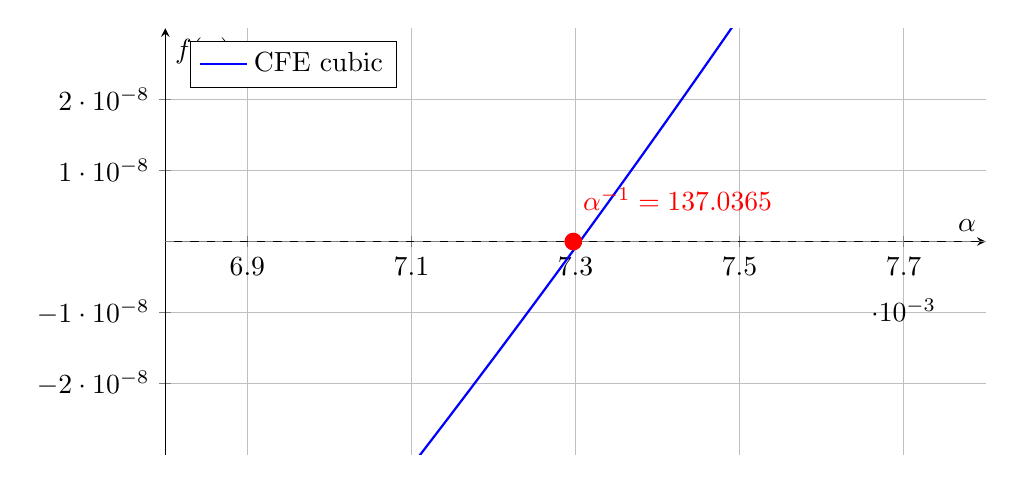
\begin{tikzpicture}
\begin{axis}[
    width=12cm, height=7cm,
    xlabel={$\alpha$},
    ylabel={$f(\alpha)$},
    xmin=0.0068, xmax=0.0078,
    ymin=-3e-8, ymax=3e-8,
    grid=major,
    axis lines=middle,
    xtick={0.0069, 0.0071, 0.0073, 0.0075, 0.0077},
    ytick={-2e-8, -1e-8, 0, 1e-8, 2e-8},
    scaled y ticks=false,
    yticklabel style={/pgf/number format/sci},
    legend pos=north west
]
    % CFE cubic
    \addplot[domain=0.0068:0.0078, samples=200, thick, blue] 
        {x^3 - 2*0.039788735773^3*x^2 - 8*4.1*0.039788735773^6*2.9439};
    \addlegendentry{CFE cubic}
    
    % Root marker
    \addplot[only marks, mark=*, mark size=3pt, red] 
        coordinates {(0.00729733, 0)};
    \node[red, above right] at (axis cs:0.00729733, 0.3e-8) 
        {$\alpha^{-1} = 137.0365$};
    
    % Zero line
    \addplot[domain=0.0068:0.0078, dashed, gray] {0};
\end{axis}
\end{tikzpicture}
\caption{The CFE has a unique positive root at $\alpha \approx 0.007297$, 
corresponding to $\alpha^{-1} \approx 137.0365$ (baseline with fixed $\phiz$).}
\label{fig:CFE}
\end{figure}

\begin{figure}[H]
\centering
\begin{tikzpicture}
\begin{groupplot}[
    group style={group size=2 by 1, horizontal sep=1.2cm},
    width=0.45\linewidth,
    height=0.36\linewidth
]
\pgfmathsetmacro{\cThree}{0.039788735772973834}
\pgfmathsetmacro{\CfeC}{3.818809423599759e-7}
\pgfmathsetmacro{\alphaRoot}{0.007297325816919221}
\pgfmathsetmacro{\alphaStar}{8.3988370919790336e-5}
\pgfmathsetmacro{\fAlphaStar}{-3.818812385889108e-7}

\nextgroupplot[
    xlabel={$\alpha$},
    ylabel={$f(\alpha)$},
    grid=major
]
\addplot[domain=0:0.02, samples=400, thick] {x^3 - 2*(\cThree^3)*x^2 - \CfeC};
\addplot[black, dashed] coordinates {(0,0) (0.02,0)};
\addplot[only marks, mark=*, mark size=2.5pt] coordinates {(\alphaRoot,0)};
\addlegendentry{root (baseline)}
\addplot[only marks, mark=square*, mark size=2.5pt] coordinates {(\alphaStar,\fAlphaStar)};
\addlegendentry{$\alpha_\ast$ (local min)}

\nextgroupplot[
    xlabel={fixed-point iteration},
    ylabel={$|\Delta\alpha|$},
    ymode=log,
    grid=major
]
\addplot+[mark=o] coordinates {
    (0,2.7017585695945706e-08)
    (1,9.9302866397459317e-14)
    (2,3.6498668384968009e-19)
    (3,1.3415048751400539e-24)
    (4,4.9306876378145135e-30)
    (5,1.8122692680605213e-35)
};
\end{groupplot}
\end{tikzpicture}
\caption{CFE uniqueness certificate (suite). Left: baseline cubic with unique root. Right: fixed-point iteration convergence.}
\label{fig:cfe-unique-suite}
\end{figure}

\begin{figure}[H]
\centering
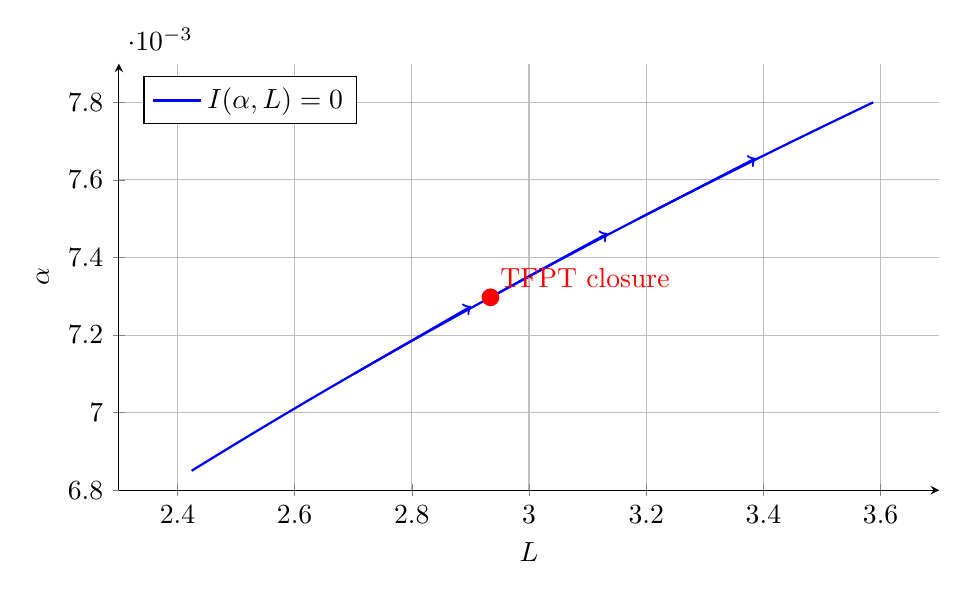
\begin{tikzpicture}
\begin{axis}[
    width=12cm, height=7cm,
    xlabel={$L$},
    ylabel={$\alpha$},
    xmin=2.3, xmax=3.7,
    ymin=0.0068, ymax=0.0079,
    grid=major,
    axis lines=left,
    legend pos=north west
]
    % Invariant surface I(\alpha,L)=0 (parametric form L(\alpha),\alpha)
    \addplot[domain=0.00685:0.0078, samples=240, thick, blue]
        ({(x^3 - 2*0.039788735773^3*x^2)/(8*4.1*0.039788735773^6)}, {x});
    \addlegendentry{$I(\alpha,L)=0$}

    % Flow direction from implicit differentiation: d\alpha/dL
    \addplot[->, thick, blue] coordinates {(2.701252,0.00710000) (2.901252,0.00727418)};
    \addplot[->, thick, blue] coordinates {(2.934229,0.00729733) (3.134229,0.00746216)};
    \addplot[->, thick, blue] coordinates {(3.187073,0.00750000) (3.387073,0.00765600)};

    % TFPT closure point (baseline)
    \addplot[only marks, mark=*, mark size=3pt, red] coordinates {(2.934224,0.00729733)};
    \node[red, above right] at (axis cs:2.934224,0.00729733) {TFPT closure};
\end{axis}
\end{tikzpicture}
\caption{Structural flow on the invariant surface $I(\alpha,L)=0$ in the $(L,\alpha)$ plane,
with arrows indicating $d\alpha/dL$ from implicit differentiation.
The marked point shows the TFPT closure solution.}
\label{fig:invariant_flow}
\end{figure}

%-----------------------------------------------------------------------------
